Šis sudarytas rekurentinis neuroninis tinklas bus taikomas kalbos modeliavime. Tiksliau tinklas bus apmokinamas prognozuoti vartotojo rašomo žodžio pabaigą ir pasiūlyti sekantį žodį (angl. \textit{Query auto-complete}).

\textbf{Duomenys}

Tinklui apmokinti bus naudojama internete rasta bet kokia knyga. Šios knygos tekstas bus suskaidytas į atskirus sakinius, kurie bus naudojami, kaip atskiri apmokymo rinkiniai.

\textbf{Apmokymas}

Kiekvienoje apmokymo iteracijoje bus paduodamas vienas sakinys. Šis sakinys suskaidytas į simbolių masyvą, kur kiekvienas simbolis bus traktuojamas, kaip viena įvesties reikšmė. Tinklo apmokymas vyksta, kai yra paduodama tam tikra simbolių seka ir pagal ją yra prognozuojamas tolimesnis tekstas. Didėjant įvesties simbolių sekai iš duotojo sakinio, prognozuojamas tolimesnis tekstas turėtų artėti arba būti panašus į esamą paduotą sakinį.

Pasirinkta tinklo apmokymo strategija:
\begin{enumerate}
  \item Iš pradžių bus paduota pirma sakinio raidė, kaip įvestis. Ši įvestis bus praleidžiama pro tinklą ir tinklas prognozuos sekančia raidę. Tuomet atliksime tinklo apmokymą, pagal prognozuojąmą raidę ir ją lyginsime su duotojo sakinio antrąją raide. Tuomet atlikę apmokymą, pagal prognozuotą raidę prognozuosime sekančią sakinio raidę. Taip ciklą kartosime tol kol įvyks vienas iš dviejų variantų:
  \begin{enumerate}
    \item jau būsime prognozavę pirmus du sakinio žodžius
    \item pasieksime sakinio pabaigą ir nebegalėsime atlikti apmokymo
  \end{enumerate}
  \begin{figure}[h!]
    \centering
  \scalebox{0.6}{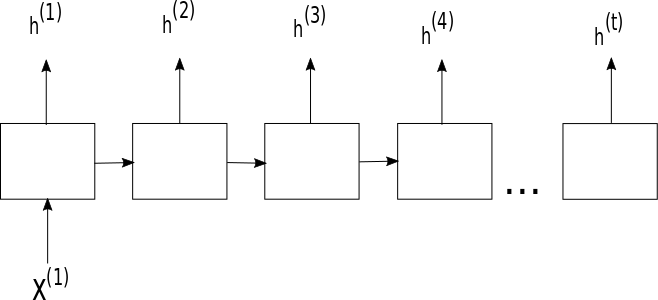
\includegraphics{images/taikymas1.png}}
  \caption{Tinklo apmokymas, kai paduodama viena sakinio raidė.}
  \label{fig:taikymas1}
  \end{figure}
  \item Toliau bus paduodamos dvi pirmos sakinio raidės, kaip įvestis. Pagal šias įvestis bus prognozuojama trečioji sakinio raidė ir tinklas bus apmokomas lyginant šią raidę su duotojo sakinio trečiąja raide. Šį ciklą taip pat kartosime tol kol įvyks vienas iš dviejų variantų paminėtų pirmame punkte.
  \begin{figure}[h!]
    \centering
  \scalebox{0.6}{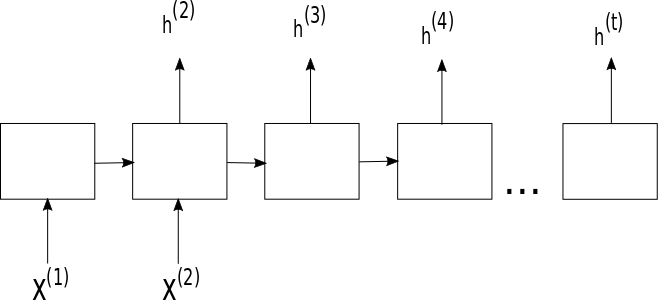
\includegraphics{images/taikymas2.png}}
  \caption{Tinklo apmokymas, kai paduodamos dvi sakinio raidės.}
  \label{fig:taikymas2}
  \end{figure}
  \item Tokiu būdu didinsime paduodamų sakinio raidžių kiekį, kaip įvestis. Pagal šias įvestis prognozuosime sekančią sakinio raidę, kurią lyginant su atitinkama duotojo sakinio raide apmokinsime tinklą. Šį ciklą kartosime iki tol kol įvyks vienas iš dviejų variantų paminėtu prieš tai buvusiuose punktuose arba paduodamų sakinio raidžių kiekis sutaps su duotuoju sakiniu.
  \begin{figure}[h!]
    \centering
  \scalebox{0.6}{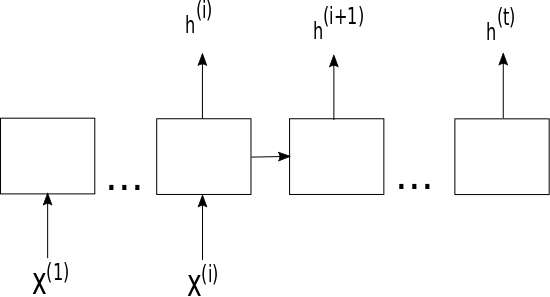
\includegraphics{images/taikymas4.png}}
  \caption{Tinklo apmokymas, kai paduodamos kelios sakinio raidės.}
  \label{fig:taikymas3}
  \end{figure}
\end{enumerate}
